% !TEX program = tectonic
% ============================================================================
% EXTERNAL PICKING DECISION ENGINE FOR SAP EWM
% Integration requirements: data, APIs and interaction for layered
% stock removal (UoM -> expiry -> storage type -> GR) computed outside EWM.
% House style follows TPO-VERSE technical notes (ParaTech Platform R&D).
% ============================================================================
\documentclass[11pt,a4paper]{article}

\usepackage[utf8]{inputenc}
\usepackage[T1]{fontenc}
\usepackage{lmodern}
\usepackage[margin=2.2cm]{geometry}
\usepackage{amsmath,amssymb}
\usepackage{xcolor}
\usepackage{tikz}
\usetikzlibrary{arrows.meta,positioning,shapes.geometric,fit,calc,backgrounds}
\usepackage{booktabs}
\usepackage{array}
\usepackage{tabularx}
\usepackage{xltabular}
\usepackage{enumitem}
\usepackage{fancyvrb}
\usepackage[most]{tcolorbox}
\usepackage{xurl}
\usepackage[hidelinks]{hyperref}
\usepackage{fancyhdr}
\usepackage{titlesec}
\usepackage{parskip}
\usepackage{caption}
\usepackage{float}
\raggedbottom
\sloppy

% ---------- Palette (shared with TPO-VERSE notes) ----------
\definecolor{inkP}{HTML}{0F172A}
\definecolor{inkM}{HTML}{64748B}
\definecolor{pxblue}{RGB}{21,67,116}
\definecolor{pxteal}{RGB}{0,128,128}
\definecolor{pxorange}{RGB}{204,102,0}
\definecolor{pxgray}{RGB}{245,246,248}
\definecolor{pxgreen}{RGB}{34,111,60}
\definecolor{pxred}{RGB}{165,42,42}

\titleformat{\section}{\Large\bfseries\color{pxblue}}{\thesection}{0.6em}{}
\titleformat{\subsection}{\large\bfseries\color{inkP}}{\thesubsection}{0.6em}{}
\pagestyle{fancy}
\fancyhf{}
\fancyhead[L]{\small\color{inkM}External Picking Decision Engine $\leftrightarrow$ SAP EWM}
\fancyhead[R]{\small\color{inkM}ParaTech Platform R\&D}
\fancyfoot[C]{\small\thepage}
\renewcommand{\headrulewidth}{0.3pt}

% ---------- Coloured JSON samples (blocks generated by json2tex.py) ----------
\DeclareCaptionType{jsonlisting}[Listing][List of Listings]
\captionsetup[jsonlisting]{skip=4pt}
\fvset{fontsize=\scriptsize}
\newcommand{\LB}{\{}\newcommand{\RB}{\}}
\newcommand{\jk}[1]{\textcolor{pxblue}{#1}}                   % key
\newcommand{\js}[1]{\textcolor{pxgreen}{#1}}                  % string value
\newcommand{\jn}[1]{\textcolor{pxorange}{#1}}                 % number
\newcommand{\jb}[1]{\textcolor{pxred}{#1}}                    % true / false / null
\newcommand{\jp}[1]{\textcolor{inkM}{#1}}                     % punctuation
\newcommand{\jc}[1]{\textcolor{pxteal}{\itshape$\triangleleft$\,#1}} % annotation
\newtcolorbox{jsonbox}[1]{enhanced, breakable, colback=pxgray, colframe=pxblue!55, boxrule=0.5pt, arc=2pt,
  left=5pt, right=5pt, top=1pt, bottom=1pt, colbacktitle=pxblue, coltitle=white,
  title={\ttfamily\footnotesize #1}, toptitle=1.5pt, bottomtitle=1.5pt, before skip=6pt, after skip=2pt}
\newcommand{\jsonlegend}{{\scriptsize\ttfamily \jk{"key"}\quad \js{"string"}\quad \jn{123}\quad
  \jb{true / false / null}\quad \jp{\{\} [] : ,}\quad \jc{annotation, not part of the payload}\par}}

% ---------- TikZ styles (shared with TPO-VERSE notes) ----------
\tikzset{
  box/.style={draw=pxblue, thick, rounded corners=2pt, fill=pxgray,
    align=center, font=\footnotesize, inner sep=4pt, minimum height=7mm},
  sys/.style={draw=pxblue, thick, rounded corners=2pt, fill=pxblue!10,
    align=center, font=\footnotesize\bfseries, inner sep=4pt, minimum height=8mm},
  newb/.style={draw=pxorange, thick, rounded corners=2pt, fill=pxorange!10,
    align=center, font=\footnotesize, inner sep=4pt, minimum height=7mm},
  ext/.style={draw=pxteal, thick, rounded corners=2pt, fill=pxteal!10,
    align=center, font=\footnotesize, inner sep=4pt, minimum height=7mm},
  data/.style={draw=pxgreen, thick, fill=pxgreen!10, align=center,
    font=\footnotesize, inner sep=4pt, minimum height=7mm, rounded corners=6pt},
  flow/.style={-{Stealth[length=2.2mm]}, thick, pxblue},
  flow2/.style={-{Stealth[length=2.2mm]}, thick, pxteal, dashed},
  flow3/.style={-{Stealth[length=2.2mm]}, thick, pxorange},
  lbl/.style={font=\scriptsize, fill=white, inner sep=1pt},
  grp/.style={draw=pxblue!35, fill=pxblue!3, rounded corners=4pt, inner sep=7pt},
  grpo/.style={draw=pxorange!45, fill=pxorange!4, rounded corners=4pt, inner sep=7pt},
  gtitle/.style={font=\scriptsize\bfseries, text=pxblue, anchor=south west, inner sep=2pt},
  gtitleo/.style={font=\scriptsize\bfseries, text=pxorange, anchor=south west, inner sep=2pt},
}

\newcolumntype{L}{>{\raggedright\arraybackslash}X}
\newcolumntype{P}[1]{>{\raggedright\arraybackslash}p{#1}}
\newcommand{\api}[1]{\texttt{#1}}
\newcommand{\verify}{\textsuperscript{\,\textit{verify}}}

\begin{document}

\begin{titlepage}
\centering\vspace*{3cm}
{\color{pxblue}\rule{\linewidth}{1.2pt}}\\[6mm]
{\Huge\bfseries External Picking Decision Engine\par}
\vspace{4mm}
{\Large Integration requirements for SAP EWM:\\data, APIs and interaction for layered stock removal\par}
\vspace{4mm}
{\color{pxblue}\rule{\linewidth}{1.2pt}}\\[2cm]
{\large ParaTech Platform R\&D Team, ParagonCorp\par}
\vspace{2mm}
{\normalsize Requirements note, October 2026 \quad$\cdot$\quad Draft v0.2\par}
\vspace{2cm}
\begin{minipage}{0.85\linewidth}
\small\textbf{Scope.} This note specifies what an external \emph{Picking Decision Engine} (PDE) needs from SAP EWM to take over
bin, batch and HU determination for outbound picking, group the resulting tasks into warehouse orders and sequence them.
It defines the two core APIs (\api{getInventoryDetails}, \api{createWOWT}), the supporting data, the interaction pattern,
non-functional requirements and a phased plan. The decision logic is the one prototyped in the
\emph{Multi-Strategy Simulation Tools} (tabs 6--7) \cite{sim}.
\end{minipage}
\vfill
\end{titlepage}

\tableofcontents
\newpage

% ============================================================================
\section{Executive Summary}
% ============================================================================
Standard EWM determines the source bin with a storage type search sequence and a stock removal rule, then groups
warehouse tasks (WTs) into warehouse orders (WOs) with WOCR \cite{saprem}. The expected logic is a four-key cascade:
\emph{UoM layer} $\rightarrow$ \emph{earliest expiry} $\rightarrow$ \emph{storage type priority} $\rightarrow$ \emph{first goods receipt},
applied order by order across a wave. Part of it fits standard Customizing; the cross-order consumption, the HU-specific
grouping and the path sequencing are easier to own, test and evolve outside EWM.

\textbf{Key observations.}
\begin{itemize}[leftmargin=*,itemsep=2pt]
  \item The search sequence alone gets keys 2 and 3 backwards: EWM searches storage type by storage type and stops when it
        has enough stock, so storage type would beat expiry. Pooling (a storage type group) is required either way \cite{saprem}.
  \item Inventory alone is not enough. The PDE also needs the \emph{demand} (ODO items), the \emph{rules} (alternative UoM,
        priorities per quantity classification, WO limits) and a \emph{layout graph} that EWM does not hold.
  \item Released warehouse APIs are reported as S/4HANA Cloud only (SAP Note 3093108); on-premise, embedded or
        decentralized EWM needs custom services \cite{note}.
\end{itemize}

\textbf{Recommendation.} Keep EWM as the system of record and executor. Expose two core APIs---\api{getInventoryDetails}
(read quants) and \api{createWOWT} (write planned WTs/WOs with fixed source data and sequence)---plus two supporting reads
and a confirmation feed. Gate go-live with a \emph{shadow-mode} phase in which the PDE plans every wave while EWM still executes
its standard result (Section~\ref{sec:roadmap}).

% ============================================================================
\section{Scope and System Context}
\label{sec:context}
% ============================================================================
\begin{table}[H]
\centering\small
\begin{tabularx}{\linewidth}{@{}P{3.2cm}L@{}}
\toprule
\textbf{In scope} & Bin/batch/HU determination for outbound picking; WT grouping into WOs (replacing WOCR for these items);
pick sequencing; multi-order waves where later orders see only the stock left by earlier ones. \\
\textbf{Out of scope} & Putaway, replenishment, physical inventory, packing logic, goods issue posting. \\
\textbf{System of record} & SAP EWM keeps stock, WT/WO documents, confirmations and postings. The PDE holds no stock of its own. \\
\textbf{Fallback} & If the PDE does not answer within the timeout, EWM creates WTs/WOs with its standard strategy and WOCR. \\
\bottomrule
\end{tabularx}
\caption{Scope of the PDE.}
\label{tab:scope}
\end{table}

\begin{figure}[htbp]
\centering
\resizebox{\linewidth}{!}{%
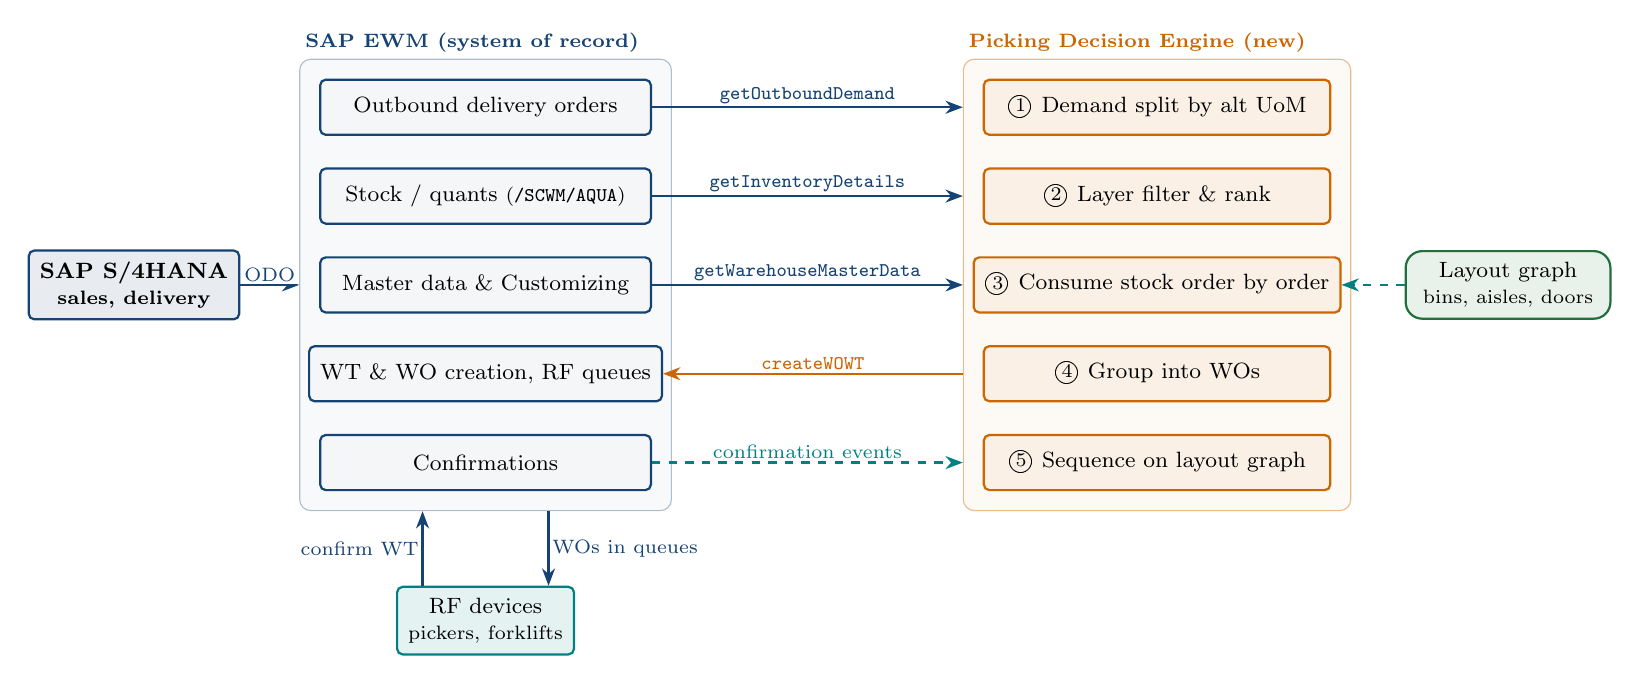
\begin{tikzpicture}[node distance=4mm and 8mm]
  % EWM
  \node[box, minimum width=4.2cm] (odo) {Outbound delivery orders};
  \node[box, below=of odo, minimum width=4.2cm] (qua) {Stock / quants \scriptsize(\texttt{/SCWM/AQUA})};
  \node[box, below=of qua, minimum width=4.2cm] (md) {Master data \& Customizing};
  \node[box, below=of md, minimum width=4.2cm] (wtwo) {WT \& WO creation, RF queues};
  \node[box, below=of wtwo, minimum width=4.2cm] (conf) {Confirmations};
  % PDE
  \node[newb, right=42mm of odo, minimum width=4.4cm] (l1) {\textcircled{\scriptsize 1} Demand split by alt UoM};
  \node[newb, below=of l1, minimum width=4.4cm] (l2) {\textcircled{\scriptsize 2} Layer filter \& rank};
  \node[newb, below=of l2, minimum width=4.4cm] (l3) {\textcircled{\scriptsize 3} Consume stock order by order};
  \node[newb, below=of l3, minimum width=4.4cm] (l4) {\textcircled{\scriptsize 4} Group into WOs};
  \node[newb, below=of l4, minimum width=4.4cm] (l5) {\textcircled{\scriptsize 5} Sequence on layout graph};
  \node[data, right=8mm of l3, minimum width=2.6cm] (graph) {Layout graph\\\scriptsize bins, aisles, doors};
  % context
  \node[sys, left=10mm of md] (erp) {SAP S/4HANA\\\scriptsize sales, delivery};
  \node[ext, below=12mm of conf] (rf) {RF devices\\\scriptsize pickers, forklifts};
  \begin{scope}[on background layer]
    \node[grp, fit=(odo)(conf)] (ge) {};
    \node[grpo, fit=(l1)(l5)] (gp) {};
    \node[gtitle] at (ge.north west) {SAP EWM (system of record)};
    \node[gtitleo] at (gp.north west) {Picking Decision Engine (new)};
  \end{scope}
  \draw[flow] (erp) -- node[lbl,above]{ODO} (ge.west |- erp);
  \draw[flow] (odo.east) -- node[lbl,above]{\api{getOutboundDemand}} (gp.west |- odo.east);
  \draw[flow] (qua.east) -- node[lbl,above]{\api{getInventoryDetails}} (gp.west |- qua.east);
  \draw[flow] (md.east) -- node[lbl,above]{\api{getWarehouseMasterData}} (gp.west |- md.east);
  \draw[flow3] (gp.west |- wtwo.east) -- node[lbl,above]{\api{createWOWT}} (wtwo.east);
  \draw[flow2] (conf.east) -- node[lbl,above]{confirmation events} (gp.west |- conf.east);
  \draw[flow2] (graph) -- (l3.east);
  \draw[flow] ([xshift=8mm]ge.south) -- node[lbl,right]{WOs in queues} ([xshift=8mm]rf.north);
  \draw[flow] ([xshift=-8mm]rf.north) -- node[lbl,left]{confirm WT} ([xshift=-8mm]ge.south);
\end{tikzpicture}}
\caption{System context. Orange blocks are new engineering. Solid arrows are synchronous calls initiated by the PDE through the
integration layer; the orange arrow is the only write into EWM; dashed arrows are events or static data.}
\label{fig:context}
\end{figure}

% ============================================================================
\section{Decision Logic}
\label{sec:logic}
% ============================================================================
For an ODO item $i$ with quantity $q_i$ in base UoM and alternative UoMs $u \in \{\mathrm{PAL},\mathrm{CAR},\mathrm{IBX},\mathrm{PC}\}$
with conversion factors $f_u$, the layer quantities are obtained greedily, largest UoM first:
\begin{equation}
n_u = \Big\lfloor \tfrac{r_u}{f_u} \Big\rfloor, \qquad r_{\mathrm{PAL}} = q_i, \qquad r_{u'} = r_u - n_u f_u \ \text{for the next smaller } u'.
\end{equation}
Within layer $u$ the candidate set is $Q_u = \{\,k : \mathrm{storedUoM}_k = u,\ \mathrm{prio}_u(\mathrm{Stype}_k)\ \text{defined},\ a_k > 0\,\}$,
ranked lexicographically by
\begin{equation}
\big(\,\mathrm{SLED}_k\uparrow,\ \ \mathrm{prio}_u(\mathrm{Stype}_k)\uparrow,\ \ \mathrm{GR}_k\uparrow\,\big),
\end{equation}
and consumed in rank order until $n_u$ is covered; the available quantity $a_k$ is reduced before the next order of the wave is planned.

\begin{enumerate}[leftmargin=*,itemsep=2pt]
\item \textbf{UoM layer.} A PAL layer only takes complete pallet HUs; an opened pallet is a CAR quant.
\item \textbf{Earliest expiry} (sort field \texttt{VFDAT} ascending \cite{vfdat}). Quants below the item's minimum remaining shelf life are excluded first.
\item \textbf{Storage type priority} from the search sequence of the layer's quantity classification, all storage types pooled.
\item \textbf{First goods receipt} (date and time).
\item \textbf{Consumption.} Orders run in a defined sequence (priority, then planned GI time).
\item \textbf{Grouping.} Full-pallet HU tasks form a forklift WO; other tasks are grouped per activity area within WO limits (WTs, weight, volume).
\item \textbf{Sequencing.} Shortest walk on the layout graph from the start point through all bins of the WO to its staging lane.
\end{enumerate}

% ============================================================================
\section{Interaction}
\label{sec:interaction}
% ============================================================================
\begin{figure}[H]
\centering
\resizebox{0.92\linewidth}{!}{%
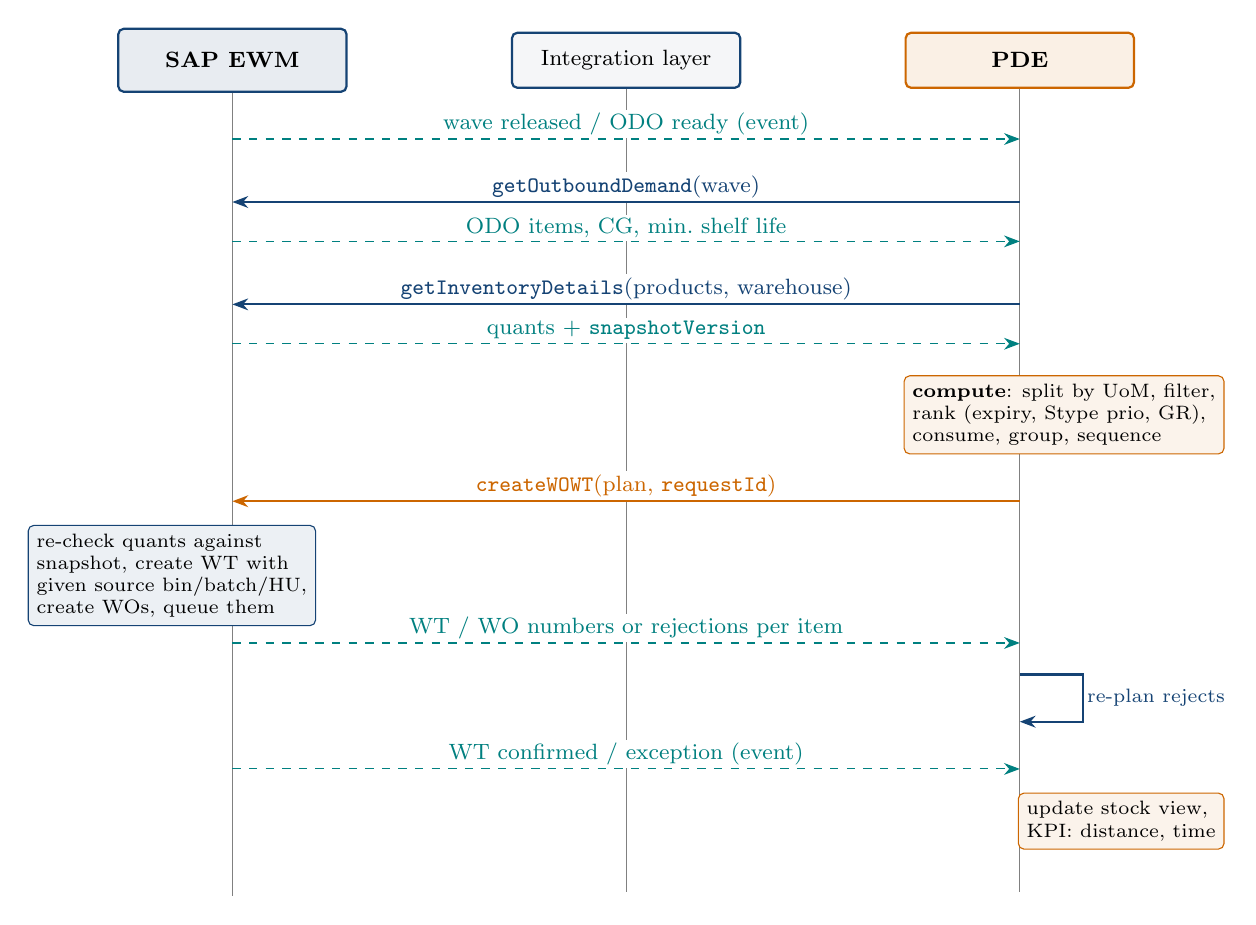
\begin{tikzpicture}[font=\footnotesize, >={Stealth[length=2mm]},
  msg/.style={->, thick, pxblue}, wr/.style={->, thick, pxorange}, ret/.style={->, dashed, pxteal},
  every node/.append style={fill=white, inner sep=1.2pt},
  note/.style={draw=pxorange, fill=pxorange!8, rounded corners=2pt, align=left, font=\scriptsize, inner sep=3pt}]
  \node[sys, minimum width=2.9cm] (e) at (0,0)  {SAP EWM};
  \node[box, minimum width=2.9cm] (i) at (5,0)  {Integration layer};
  \node[newb, minimum width=2.9cm, font=\footnotesize\bfseries] (p) at (10,0) {PDE};
  \foreach \n in {e,i,p} \draw[gray] (\n.south) -- ++(0,-10.2);
  \draw[ret] (0,-1.0) -- node[above]{wave released / ODO ready (event)} (10,-1.0);
  \draw[msg] (10,-1.8) -- node[above]{\api{getOutboundDemand}(wave)} (0,-1.8);
  \draw[ret] (0,-2.3) -- node[above]{ODO items, CG, min.\ shelf life} (10,-2.3);
  \draw[msg] (10,-3.1) -- node[above]{\api{getInventoryDetails}(products, warehouse)} (0,-3.1);
  \draw[ret] (0,-3.6) -- node[above]{quants + \texttt{snapshotVersion}} (10,-3.6);
  \node[note, anchor=north east] at (12.6,-4.0) {\textbf{compute}: split by UoM, filter,\\rank (expiry, Stype prio, GR),\\consume, group, sequence};
  \draw[wr] (10,-5.6) -- node[above]{\api{createWOWT}(plan, \texttt{requestId})} (0,-5.6);
  \node[note, draw=pxblue, fill=pxblue!8, anchor=north west] at (-2.6,-5.9) {re-check quants against\\snapshot, create WT with\\given source bin/batch/HU,\\create WOs, queue them};
  \draw[ret] (0,-7.4) -- node[above]{WT / WO numbers or rejections per item} (10,-7.4);
  \draw[msg] (10,-7.8) -- ++(0.8,0) |- node[pos=0.25, right, font=\scriptsize]{re-plan rejects} (10,-8.4);
  \draw[ret] (0,-9.0) -- node[above]{WT confirmed / exception (event)} (10,-9.0);
  \node[note, anchor=north east] at (12.6,-9.3) {update stock view,\\KPI: distance, time};
\end{tikzpicture}}
\caption{End-to-end interaction for one wave. Blue: reads; orange: the write; dashed teal: responses and events.}
\label{fig:sequence}
\end{figure}

% ============================================================================
\section{API 1 -- \texorpdfstring{\api{getInventoryDetails}}{getInventoryDetails}}
\label{sec:api1}
% ============================================================================
\textbf{Purpose:} available stock per quant for the products in the plan. \textbf{Call:} \texttt{GET}, filtered by warehouse and
product list (optionally storage types, stock type). \textbf{Volume:} one call per wave, paged. \textbf{Freshness:} near real time;
the response carries a snapshot version used by \api{createWOWT}. Table~\ref{tab:api1} lists the fields, using the EWM structure terms of \cite{sapstruct}; Listing~\ref{lst:api1} shows a response.

{\small
\begin{xltabular}{\linewidth}{@{}P{3.4cm}P{2.0cm}P{3.7cm}L@{}}
\caption{\api{getInventoryDetails} response fields (one row per quant).}\label{tab:api1}\\
\toprule
\textbf{Field} & \textbf{Type} & \textbf{EWM source\verify} & \textbf{Used for} \\
\midrule
\endfirsthead
\toprule
\textbf{Field} & \textbf{Type} & \textbf{EWM source\verify} & \textbf{Used for} \\
\midrule
\endhead
\texttt{warehouse} & char 4 & \texttt{LGNUM} & scope \\
\texttt{quantId} & GUID & quant / stock GUID & reference in \api{createWOWT} \\
\texttt{product} & char 40 & \texttt{MATNR} & matching demand \\
\texttt{batch} & char 10 & \texttt{CHARG} & traceability, batch-specific demand \\
\texttt{sled} & date & shelf-life expiration (\texttt{VFDAT}) & key 2, min.\ shelf-life check \\
\texttt{grDateTime} & timestamp & GR date/time (\texttt{WDATU}) & key 4 \\
\texttt{bin} & char 18 & \texttt{LGPLA} & source bin, layout lookup \\
\texttt{storageType} & char 4 & \texttt{LGTYP} & key 3, layer eligibility \\
\texttt{storageSection} & char 4 & \texttt{LGBER} & reporting, optional rules \\
\texttt{activityArea} & char 4 & activity area of the bin & grouping \\
\texttt{qtyAvailable}, \texttt{baseUoM} & dec, char 3 & physical minus open removal qty & consumption \\
\texttt{qtyPhysical}, \texttt{qtyOpenRemoval} & dec & quant / open WTs & transparency \\
\texttt{storedUoM}, \texttt{storedQty} & char 3, dec & stock-specific UoM / packaging & layer filter (PAL, CAR, IBX, PC) \\
\texttt{huId}, \texttt{huType}, \texttt{isFullHU} & char 20, char 4, bool & HU of the quant & PAL layer, HU WT \\
\texttt{stockType}, \texttt{owner}, \texttt{entitled} & char & stock category fields & only unrestricted, own stock \\
\texttt{blocked} & bool & bin / quant block indicators & exclude \\
\texttt{changedAt} & timestamp & last change & concurrency check \\
\midrule
\multicolumn{4}{@{}l}{\textit{Envelope:} \texttt{snapshotVersion}, \texttt{generatedAt}, paging token \texttt{next}.} \\
\bottomrule
\end{xltabular}}

% JSON:api1 (generated by json2tex.py - edit the script, not this block)
\begin{jsonbox}{GET /inventory?warehouse=WH01\&products=E,F,G \quad$\rightarrow$\quad 200 OK}
\begin{Verbatim}[commandchars=\\\{\}]
\jp{\LB}
  \jk{"warehouse"}\jp{:} \js{"WH01"}\jp{,}
  \jk{"snapshotVersion"}\jp{:} \js{"2026-10-21T08:15:02Z#4711"}\jp{,}         \jc{echo it in createWOWT}
  \jk{"generatedAt"}\jp{:} \js{"2026-10-21T08:15:02Z"}\jp{,}
  \jk{"next"}\jp{:} \jb{null}\jp{,}                                           \jc{paging token, null = last page}
  \jk{"quants"}\jp{:} \jp{[}
    \jp{\LB}
      \jk{"quantId"}\jp{:} \js{"6f1c..."}\jp{,}
      \jk{"product"}\jp{:} \js{"E"}\jp{,}
      \jk{"batch"}\jp{:} \js{"E2611-30"}\jp{,}
      \jk{"sled"}\jp{:} \js{"2026-11-30"}\jp{,}                               \jc{key 2: earliest expiry}
      \jk{"grDateTime"}\jp{:} \js{"2026-09-10T07:42:00Z"}\jp{,}               \jc{key 4: first goods receipt}
      \jk{"bin"}\jp{:} \js{"06-L9"}\jp{,}                                     \jc{source bin, node in layout graph}
      \jk{"storageType"}\jp{:} \js{"0030"}\jp{,}                              \jc{key 3: priority per layer}
      \jk{"storageSection"}\jp{:} \js{"0001"}\jp{,}
      \jk{"activityArea"}\jp{:} \js{"PCK-R"}\jp{,}                            \jc{WO grouping}
      \jk{"qtyAvailable"}\jp{:} \jn{500}\jp{,}                                \jc{physical - open removal, base UoM}
      \jk{"baseUoM"}\jp{:} \js{"PC"}\jp{,}
      \jk{"storedUoM"}\jp{:} \js{"PAL"}\jp{,}                                 \jc{key 1: UoM layer filter}
      \jk{"storedQty"}\jp{:} \jn{1}\jp{,}
      \jk{"huId"}\jp{:} \js{"P-1002"}\jp{,}
      \jk{"huType"}\jp{:} \js{"EUR"}\jp{,}
      \jk{"isFullHU"}\jp{:} \jb{true}\jp{,}                                   \jc{only full HUs enter the PAL layer}
      \jk{"stockType"}\jp{:} \js{"F2"}\jp{,}
      \jk{"blocked"}\jp{:} \jb{false}\jp{,}                                   \jc{true = never a candidate}
      \jk{"changedAt"}\jp{:} \js{"2026-10-20T16:03:11Z"}                 \jc{concurrency check}
    \jp{\RB}\jp{,}
    \jp{\LB}
      \jk{"quantId"}\jp{:} \js{"9a07..."}\jp{,}                               \jc{second quant: fields as above}
      \jk{"product"}\jp{:} \js{"E"}\jp{,}
      \jk{"batch"}\jp{:} \js{"E2611-10"}\jp{,}
      \jk{"sled"}\jp{:} \js{"2026-11-10"}\jp{,}
      \jk{"grDateTime"}\jp{:} \js{"2026-08-12T09:10:00Z"}\jp{,}
      \jk{"bin"}\jp{:} \js{"04-R4"}\jp{,}
      \jk{"storageType"}\jp{:} \js{"0020"}\jp{,}
      \jk{"qtyAvailable"}\jp{:} \jn{200}\jp{,}
      \jk{"storedUoM"}\jp{:} \js{"CAR"}\jp{,}
      \jk{"storedQty"}\jp{:} \jn{4}\jp{,}
      \jk{"huId"}\jp{:} \jb{null}\jp{,}
      \jk{"isFullHU"}\jp{:} \jb{false}
    \jp{\RB}
  \jp{]}
\jp{\RB}
\end{Verbatim}
\end{jsonbox}
\jsonlegend
\captionof{jsonlisting}{\api{getInventoryDetails} response excerpt (data from the simulation, tab 7).}\label{lst:api1}
% END JSON:api1

% ============================================================================
\section{API 2 -- \texorpdfstring{\api{createWOWT}}{createWOWT}}
\label{sec:api2}
% ============================================================================
\textbf{Purpose:} create the planned WTs with fixed source data and group them into WOs in the given sequence.
\textbf{Call:} \texttt{POST}, idempotent on \texttt{requestId}. \textbf{Atomicity:} all-or-nothing per WO; other WOs of the same
request may succeed. Table~\ref{tab:api2} lists the structure; Listings~\ref{lst:api2} and~\ref{lst:api2r} show a request and its response.

{\small
\begin{xltabular}{\linewidth}{@{}P{4.4cm}L@{}}
\caption{\api{createWOWT} request and response structure.}\label{tab:api2}\\
\toprule
\multicolumn{2}{@{}l}{\textbf{Request header}} \\
\midrule
\endfirsthead
\toprule
\textbf{Field} & \textbf{Meaning} \\
\midrule
\endhead
\texttt{requestId}, \texttt{planRunId} & idempotency key; plan identifier for audit and KPIs \\
\texttt{warehouse}, \texttt{snapshotVersion} & scope; inventory version the plan was computed on \\
\midrule
\multicolumn{2}{@{}l}{\textbf{Per warehouse order}} \\
\midrule
\texttt{woRef}, \texttt{woType} & external id; \texttt{PICK} or \texttt{FULL\_HU} \\
\texttt{queue}, \texttt{resourceType} & RF queue and resource (picker, forklift) \\
\texttt{activityArea}, \texttt{consolidationGroup} & grouping attributes stored on the WO \\
\texttt{destination} & staging bin / lane / door \\
\texttt{plannedDistance}, \texttt{plannedDuration} & KPIs from the PDE \\
\midrule
\multicolumn{2}{@{}l}{\textbf{Per warehouse task (ordered list inside the WO)}} \\
\midrule
\texttt{wtRef}, \texttt{seqNo} & external id; pick sequence in the WO \\
\texttt{odo}, \texttt{odoItem} & warehouse request reference \\
\texttt{product}, \texttt{batch}, \texttt{qty}, \texttt{uom} & what to pick, in the layer UoM (e.g.\ 2 CAR) \\
\texttt{sourceBin}, \texttt{sourceHU}, \texttt{quantId} & fixed source; \texttt{sourceHU} makes it an HU WT \\
\texttt{processType}, \texttt{destinationBin} & warehouse process type (outbound pick\verify) and staging bin \\
\texttt{layerTrace} & UoM layer and deciding key, for audit \\
\midrule
\multicolumn{2}{@{}l}{\textbf{Response}} \\
\midrule
per WO & EWM WO number, or the reject code of the first failing WT \\
per WT & EWM WT number, or one of \texttt{STOCK\_CHANGED}, \texttt{QTY\_INSUFFICIENT}, \texttt{BIN\_BLOCKED},
  \texttt{ITEM\_ALREADY\_PLANNED}, \texttt{UOM\_INVALID}, \texttt{AUTH} \\
\bottomrule
\end{xltabular}}

% JSON:api2 (generated by json2tex.py - edit the script, not this block)
\begin{jsonbox}{POST /warehouse-orders \quad Idempotency-Key: 8f2c4e1a-...}
\begin{Verbatim}[commandchars=\\\{\}]
\jp{\LB}
  \jk{"requestId"}\jp{:} \js{"8f2c4e1a-..."}\jp{,}                            \jc{idempotency key}
  \jk{"planRunId"}\jp{:} \js{"PDE-20261021-0815-07"}\jp{,}
  \jk{"warehouse"}\jp{:} \js{"WH01"}\jp{,}
  \jk{"snapshotVersion"}\jp{:} \js{"2026-10-21T08:15:02Z#4711"}\jp{,}         \jc{from getInventoryDetails}
  \jk{"warehouseOrders"}\jp{:} \jp{[}
    \jp{\LB}
      \jk{"woRef"}\jp{:} \js{"PDE-WO-3"}\jp{,}
      \jk{"woType"}\jp{:} \js{"FULL_HU"}\jp{,}                                \jc{FULL_HU = forklift WO}
      \jk{"queue"}\jp{:} \js{"FORKLIFT"}\jp{,}
      \jk{"resourceType"}\jp{:} \js{"FL"}\jp{,}
      \jk{"activityArea"}\jp{:} \js{"PCK-R"}\jp{,}
      \jk{"consolidationGroup"}\jp{:} \js{"CG-ST17"}\jp{,}
      \jk{"destination"}\jp{:} \js{"9010-LANE-124"}\jp{,}                     \jc{GI staging lane of the delivery}
      \jk{"plannedDistance"}\jp{:} \jn{186}\jp{,}                             \jc{metres on the layout graph}
      \jk{"plannedDuration"}\jp{:} \jn{240}\jp{,}                             \jc{seconds}
      \jk{"tasks"}\jp{:} \jp{[}
        \jp{\LB}
          \jk{"wtRef"}\jp{:} \js{"PDE-WT-1"}\jp{,}
          \jk{"seqNo"}\jp{:} \jn{1}\jp{,}                                     \jc{pick order inside the WO}
          \jk{"odo"}\jp{:} \js{"PM#124"}\jp{,}
          \jk{"odoItem"}\jp{:} \jn{10}\jp{,}
          \jk{"product"}\jp{:} \js{"E"}\jp{,}
          \jk{"batch"}\jp{:} \js{"E2611-30"}\jp{,}
          \jk{"qty"}\jp{:} \jn{1}\jp{,}
          \jk{"uom"}\jp{:} \js{"PAL"}\jp{,}                                   \jc{layer UoM, not base UoM}
          \jk{"sourceBin"}\jp{:} \js{"06-L9"}\jp{,}
          \jk{"sourceHU"}\jp{:} \js{"P-1002"}\jp{,}                           \jc{set = HU WT, pallet not opened}
          \jk{"quantId"}\jp{:} \js{"6f1c..."}\jp{,}                           \jc{re-checked against the snapshot}
          \jk{"destinationBin"}\jp{:} \js{"9010-LANE-124"}\jp{,}
          \jk{"layerTrace"}\jp{:} \js{"PAL; tie on expiry with 09-L2; decided at Stype prio"}  \jc{audit: why this quant}
        \jp{\RB}
      \jp{]}
    \jp{\RB}
  \jp{]}
\jp{\RB}
\end{Verbatim}
\end{jsonbox}
\jsonlegend
\captionof{jsonlisting}{\api{createWOWT} request excerpt: the forklift WO of delivery PM\#124.}\label{lst:api2}
% END JSON:api2

% JSON:api2r (generated by json2tex.py - edit the script, not this block)
\begin{jsonbox}{200 OK \quad (partial success: WOs are all-or-nothing)}
\begin{Verbatim}[commandchars=\\\{\}]
\jp{\LB}
  \jk{"requestId"}\jp{:} \js{"8f2c4e1a-..."}\jp{,}
  \jk{"warehouseOrders"}\jp{:} \jp{[}
    \jp{\LB}
      \jk{"woRef"}\jp{:} \js{"PDE-WO-3"}\jp{,}
      \jk{"status"}\jp{:} \js{"CREATED"}\jp{,}
      \jk{"ewmWO"}\jp{:} \js{"20004711"}\jp{,}                                \jc{EWM warehouse order number}
      \jk{"tasks"}\jp{:} \jp{[}
        \jp{\LB}
          \jk{"wtRef"}\jp{:} \js{"PDE-WT-1"}\jp{,}
          \jk{"status"}\jp{:} \js{"CREATED"}\jp{,}
          \jk{"ewmWT"}\jp{:} \js{"100045671"}                            \jc{EWM warehouse task number}
        \jp{\RB}
      \jp{]}
    \jp{\RB}\jp{,}
    \jp{\LB}
      \jk{"woRef"}\jp{:} \js{"PDE-WO-2"}\jp{,}
      \jk{"status"}\jp{:} \js{"REJECTED"}\jp{,}                               \jc{whole WO rolled back}
      \jk{"tasks"}\jp{:} \jp{[}
        \jp{\LB}
          \jk{"wtRef"}\jp{:} \js{"PDE-WT-7"}\jp{,}
          \jk{"status"}\jp{:} \js{"REJECTED"}\jp{,}
          \jk{"reason"}\jp{:} \js{"STOCK_CHANGED"}\jp{,}                      \jc{PDE re-plans this item only}
          \jk{"detail"}\jp{:} \js{"04-R4: available 2 CAR, planned 3 CAR"}
        \jp{\RB}
      \jp{]}
    \jp{\RB}
  \jp{]}
\jp{\RB}
\end{Verbatim}
\end{jsonbox}
\jsonlegend
\captionof{jsonlisting}{\api{createWOWT} response: one WO created, one rejected because its stock changed after the snapshot.}\label{lst:api2r}
% END JSON:api2r

% ============================================================================
\section{Supporting Data Contracts}
\label{sec:contracts}
% ============================================================================
The two core APIs are not enough on their own: the PDE also needs the demand, the rules and the layout (Table~\ref{tab:contracts}).

{\small
\begin{xltabular}{\linewidth}{@{}P{4.3cm}L P{2.0cm}@{}}
\caption{Supporting data contracts.}\label{tab:contracts}\\
\toprule
\textbf{Source} & \textbf{Feed} & \textbf{Cadence} \\
\midrule
\endfirsthead
\toprule
\textbf{Source} & \textbf{Feed} & \textbf{Cadence} \\
\midrule
\endhead
\api{getOutboundDemand} & ODO number and item, product, quantity in base UoM, requested batch, min.\ remaining shelf life,
  consolidation group, ship-to, route/door, planned GI time, priority, wave & per wave \\
\api{getWarehouseMasterData} & alternative UoM conversions and quantity classification per UoM; batch and shelf-life flags;
  storage types with role, full-HU removal and mixed-storage flags; search sequence and priority per quantity classification;
  WO limits per activity area; queues and resources & daily + on change \\
Layout graph & per bin: x/y (or aisle--stack--level), access point on the aisle, bin type; aisle segments, one-way and
  forklift-only restrictions; start points, staging lanes, doors. Not standard EWM data: maintained once and versioned & on change \\
Confirmation events & WT confirmed (actual quantity, actual bin, exceptions), WO completed, stock changes outside the plan & streaming \\
\bottomrule
\end{xltabular}}

% ============================================================================
\section{Exposing the APIs from SAP}
\label{sec:sap}
% ============================================================================
\begin{table}[H]
\centering\small
\begin{tabularx}{\linewidth}{@{}P{2.4cm}LL@{}}
\toprule
& \textbf{SAP S/4HANA Cloud} & \textbf{On-premise / embedded or decentralized EWM} \\
\midrule
Read stock & released OData APIs (warehouse stock, storage bin)\verify & custom OData/RFC on the quant view (\texttt{/SCWM/AQUA}) \\
Read demand & warehouse outbound delivery order API\verify & custom service on ODO items \\
Create WT/WO & warehouse order and task API\verify; check that creation with a fixed source is supported & custom service: create WTs with explicit
  source bin, batch and HU, then build WOs in the given sequence; trigger via PPF action or BAdI before WOCR \\
Events & SAP Event Mesh / business events\verify & custom event on WT confirmation \\
\bottomrule
\end{tabularx}
\caption{Implementation options by deployment model.}
\label{tab:sap}
\end{table}

A community thread cites SAP Note 3093108: the released warehouse APIs are meant for S/4HANA Cloud and are not supported for
embedded or decentralized EWM \cite{note}. A comparable external pick optimizer hooks in after WT creation and leaves the
write-back to the customer project \cite{optioryx}. Confirm the deployment model first; for on-premise, plan for custom services.

% ============================================================================
\section{Non-Functional Requirements}
\label{sec:nfr}
% ============================================================================
\begin{table}[H]
\centering\small
\begin{tabularx}{\linewidth}{@{}P{3.0cm}L P{3.6cm}@{}}
\toprule
\textbf{Requirement} & \textbf{Specification} & \textbf{Acceptance} \\
\midrule
Latency & one wave ($\le$\,500 items) planned and written back within 10\,s & p95 $\le$ 10\,s in load test \\
Fallback & timeout or error $\rightarrow$ EWM standard strategy and WOCR & no wave left unplanned \\
Consistency & \api{createWOWT} re-checks each quant against the snapshot; rejects only the affected WT/WO; PDE re-plans those items & zero double allocations \\
Idempotency & a repeated \texttt{requestId} returns the first result and creates nothing new & replay test passes \\
Security & OAuth 2.0 client credentials, technical user restricted to the warehouse, TLS & security review signed off \\
Audit & store \texttt{planRunId}, inputs, ranking trace and document numbers for 90 days & any WT traceable to its rank \\
Monitoring & success, reject and fallback rates; planned vs.\ actual pick distance & dashboard live before pilot \\
\bottomrule
\end{tabularx}
\caption{Non-functional requirements and acceptance criteria.}
\label{tab:nfr}
\end{table}

% ============================================================================
\section{Roadmap}
\label{sec:roadmap}
% ============================================================================
\begin{figure}[H]
\centering
\resizebox{\linewidth}{!}{%
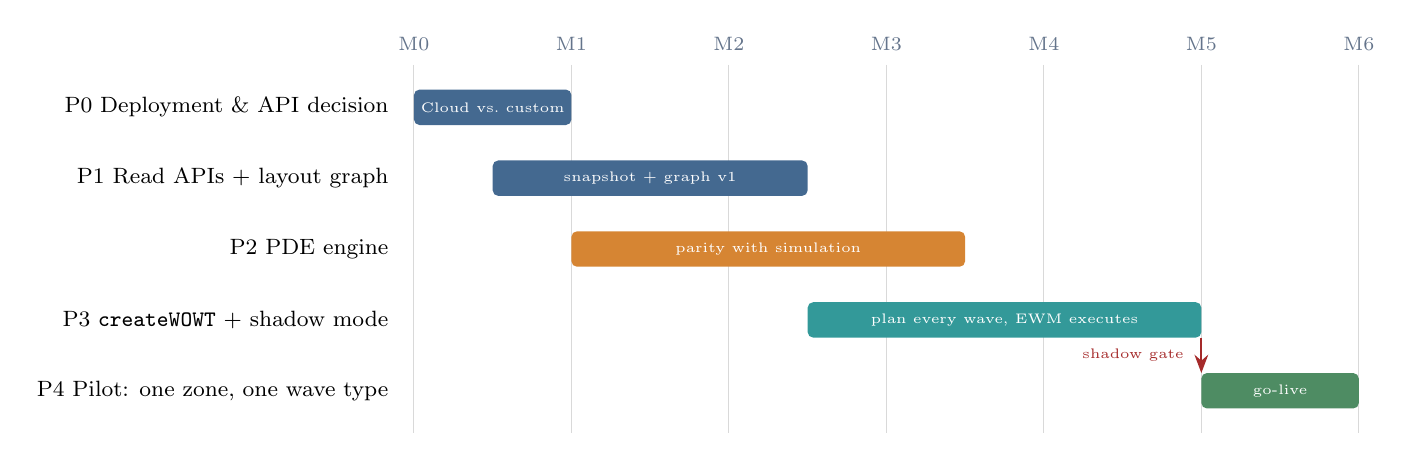
\begin{tikzpicture}[x=1.0cm, y=-0.9cm]
  \foreach \x/\t in {0/{M0},2/{M1},4/{M2},6/{M3},8/{M4},10/{M5},12/{M6}}{
    \node[font=\scriptsize, text=inkM] at (\x,-0.3) {\t};
    \draw[gray!30] (\x,0) -- (\x,5.2);}
  \node[anchor=east, font=\footnotesize] at (-0.2,0.6) {P0 Deployment \& API decision};
  \node[anchor=east, font=\footnotesize] at (-0.2,1.6) {P1 Read APIs + layout graph};
  \node[anchor=east, font=\footnotesize] at (-0.2,2.6) {P2 PDE engine};
  \node[anchor=east, font=\footnotesize] at (-0.2,3.6) {P3 \texttt{createWOWT} + shadow mode};
  \node[anchor=east, font=\footnotesize] at (-0.2,4.6) {P4 Pilot: one zone, one wave type};
  \fill[pxblue!80, rounded corners=2pt] (0,0.35) rectangle (2,0.85);
  \fill[pxblue!80, rounded corners=2pt] (1,1.35) rectangle (5,1.85);
  \fill[pxorange!80, rounded corners=2pt] (2,2.35) rectangle (7,2.85);
  \fill[pxteal!80, rounded corners=2pt] (5,3.35) rectangle (10,3.85);
  \fill[pxgreen!80, rounded corners=2pt] (10,4.35) rectangle (12,4.85);
  \node[font=\tiny, text=white] at (1,0.6) {Cloud vs.\ custom};
  \node[font=\tiny, text=white] at (3,1.6) {snapshot + graph v1};
  \node[font=\tiny, text=white] at (4.5,2.6) {parity with simulation};
  \node[font=\tiny, text=white] at (7.5,3.6) {plan every wave, EWM executes};
  \node[font=\tiny, text=white] at (11,4.6) {go-live};
  \draw[pxred, thick, -{Stealth}] (10,3.85) -- (10,4.35);
  \node[font=\tiny, text=pxred, anchor=east] at (9.9,4.1) {shadow gate};
\end{tikzpicture}}
\caption{Indicative phasing (months). The shadow gate: for four weeks of real waves the PDE plan must be feasible
($\ge$\,99\,\% of WTs accepted) and must not lengthen the pick distance against the EWM standard result before it is allowed to write.}
\label{fig:roadmap}
\end{figure}

\begin{table}[H]
\centering\small
\begin{tabularx}{\linewidth}{@{}l X X@{}}
\toprule
\textbf{Phase} & \textbf{Deliverable} & \textbf{Exit criterion}\\
\midrule
P0 & Deployment model confirmed; standard vs.\ custom API decision; field mapping signed off & Table~\ref{tab:sap} closed \\
P1 & \api{getInventoryDetails}, \api{getOutboundDemand}, \api{getWarehouseMasterData}; layout graph v1 & Snapshot matches EWM stock overview for one day \\
P2 & PDE engine: layers, ranking, consumption, grouping, sequencing & Same picks as the simulation for the tab 6--7 test cases \cite{sim} \\
P3 & \api{createWOWT}, confirmation feed, shadow mode & Shadow gate passed (Fig.~\ref{fig:roadmap}) \\
P4 & Pilot in one activity area and one wave type & Pick distance and FEFO compliance at or above baseline \\
\bottomrule
\end{tabularx}
\caption{Phases and exit criteria.}
\label{tab:phases}
\end{table}

\subsection{Risks and mitigations}
\begin{itemize}[leftmargin=*,itemsep=2pt]
  \item \textbf{No standard write API for fixed-source WTs} -- decide in P0; budget a custom service wrapping WT creation.
  \item \textbf{Stock changes between read and write} -- snapshot version plus per-quant re-check; reject and re-plan only the affected items.
  \item \textbf{Stored UoM missing on quants} -- derive it from HU type and quantity in P1, or activate stock-specific UoM.
  \item \textbf{Layout graph drifts from the floor} -- version it, validate every bin in EWM exists in the graph, re-check after re-slotting.
  \item \textbf{Two sources of truth for rules} -- priorities and UoM data are read from EWM Customizing, never retyped in the PDE.
\end{itemize}

\subsection{Open points}
\begin{itemize}[leftmargin=*,itemsep=2pt]
  \item Deployment model (S/4HANA Cloud, embedded or decentralized EWM).
  \item Can EWM create WTs with a fixed source quant and keep the external WO grouping and sequence unchanged?
  \item Owner of the layout graph and of the storage type priorities per quantity classification.
  \item Behaviour when a layer runs short: next smaller UoM, or shortage on the ODO item.
\end{itemize}

% ============================================================================
\section{Conclusion}
% ============================================================================
The layered logic is small and deterministic; what makes it an integration project is the data around it. With two core APIs,
two supporting reads, a versioned layout graph and a shadow gate before the first write, EWM keeps control of stock and execution
while the PDE owns the decision---testable against the simulation and replaceable without touching EWM Customizing.

\vspace{4mm}
\noindent\textbf{Source note.} The decision logic and the sample data come from the Multi-Strategy Simulation Tools and the companion
logic note \cite{sim}. API names marked \textit{verify} and the EWM field mapping are proposals to be confirmed against the target
system; they are not tested interfaces.

\begin{thebibliography}{9}
\bibitem{saprem} SAP Learning, ``Applying the stock removal strategies,'' \emph{Basic Customizing in SAP S/4HANA EWM}. [Online]. Available: \url{https://learning.sap.com/courses/basic-customizing-in-sap-s-4hana-ewm/applying-the-stock-removal-strategies}
\bibitem{sapstruct} SAP Learning, ``Outlining warehouse structures,'' \emph{Processes in SAP S/4HANA EWM}. [Online]. Available: \url{https://learning.sap.com/courses/processes-in-sap-s-4hana-ewm/outlining-warehouse-structures}
\bibitem{vfdat} SAP Community, ``EWM stock removal strategies,'' Q\&A, Feb.~2016. [Online]. Available: \url{https://community.sap.com/t5/supply-chain-management-q-a/ewm-stock-removal-strategies/qaq-p/11464648}
\bibitem{note} SAP Community, ``Warehouse order API usage for mobile app,'' Q\&A citing SAP Note 3093108, Nov.~2023. [Online]. Available: \url{https://community.sap.com/t5/technology-q-a/warehouse-order-api-usage-for-mobile-app/qaq-p/12767484}
\bibitem{optioryx} Optioryx, ``Pulse Pick: SAP EWM integration,'' documentation. [Online]. Available: \url{https://docs.optioryx.com/pulse-pick/integrations/sap-ewm}
\bibitem{sim} ParaTech Platform R\&D, ``Multi-Strategy Simulation Tools'' (\texttt{ewm-wocr-animation.html}) and ``Layered stock removal logic -- SAP EWM'' (\texttt{ewm-layered-stock-removal-logic.md}), internal, Oct.~2026.
\end{thebibliography}

\end{document}
